
\section{The Problem}
\label{sec:problem}

In this section, we motivate the need for resilient adaptive indexing in modern applications.
We first demonstrate the main advantages that existing adaptive indexing
techniques bring and then we highlight the core non-resilience problems that appear
when dealing with long strings of exploratory queries and continuous updates.
We use the original database cracking technique to highlight these benefits
and shortcomings of adaptive indexing. In Section \ref{sec:experiments},
we show that the same properties are still true for more complex adaptive indexing techniques
that were introduced more recently such as 
stochastic cracking \cite{StochasticCracking}, adaptive merging \cite{GK10b}  
and hybrid adaptive indexing \cite{AdaptiveIndexing}.


\subsection{Adaptive Behavior}
The main power of original database cracking is its ability to self-organize
automatically and at low cost.

The former feature (automatic self-organization) is crucial because it eschews the need for special decision-making as to when
the system should perform self-organizing actions;
the system self-organizes \emph{continuously} by default.
Apart from conferring benefits of efficiency and hands-free convenience in workload analysis,
such automatic self-organization also brings instant, online adaptation in response to a changing workload,
without delays.
In effect, there is no performance penalty due to having an unsuitable physical design
for a prolonged time period.

The latter feature (low cost) is also a powerful property that sets cracking apart
from approaches such as online indexing. This derives
from the ability to provide incremental and partial indexing integrated in an efficient way
\emph{inside} the database kernel.

\begin{figure}[t]
\hspace{-1em}
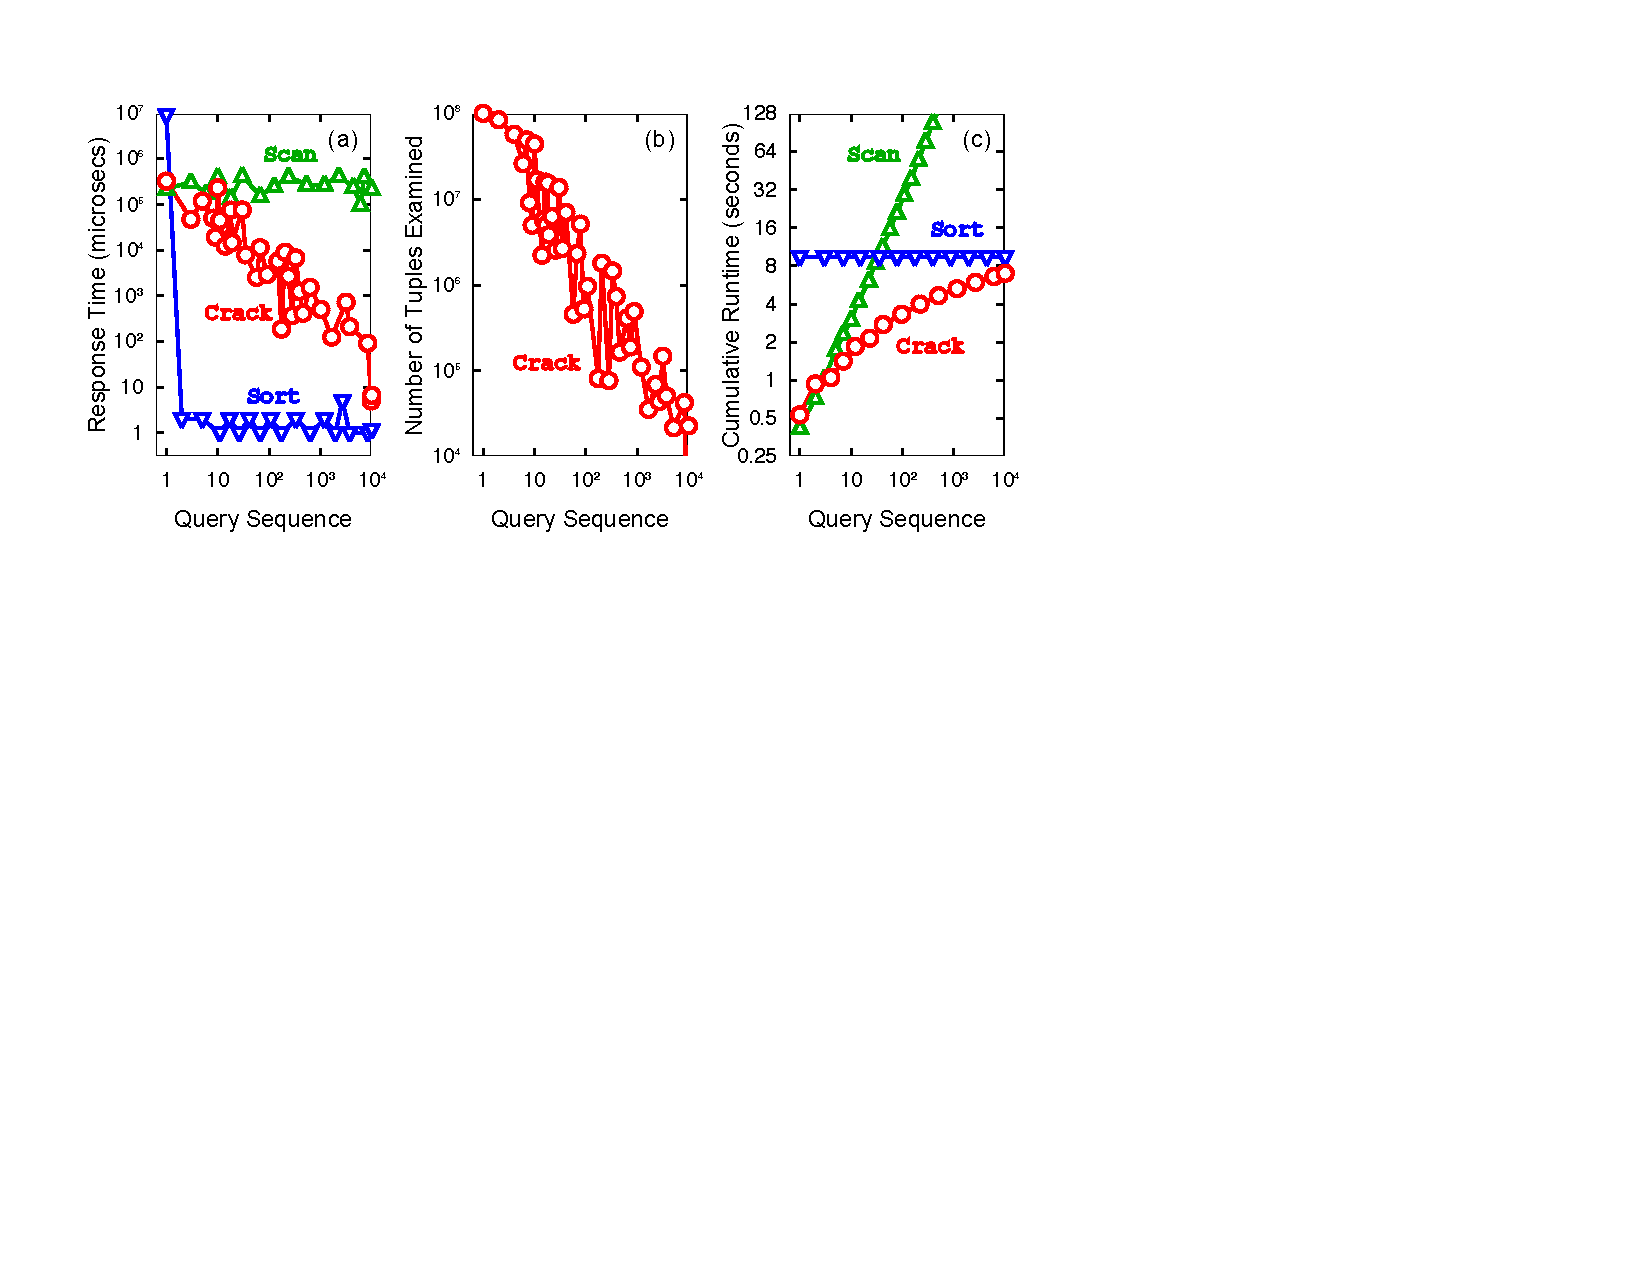
\includegraphics[width=1.05\columnwidth]{graphs/figure2.pdf}%
\vspace{-1em}
\caption{Adaptive behavior benefits of adaptive indexing.}
\vspace{-2em}
\label{F:BasicPerQuery}
\end{figure}

\textbf{Cracking Continuous Adaptation.}
As we have seen in the example of Figure \ref{F:CrackExample},
cracking feeds from the select operator, using the selection predicates to drive the way data is stored.
This way, after each query, data is clustered in a way such that the qualifying values for the
respective select operator are in a contiguous area in the attribute column. 
The more queries are processed, the more knowledge and structure
are introduced; this is how cracking achieves instant adaptation.



\textbf{Cracking Cost.}
Let us now discuss the cost of cracking, i.e., the cost to run the select operator, which includes the cost
for identifying what kind of physical reorganizations are needed and performing such reorganizations.

A cracking DBMS maintains indexes, showing which piece of the array holds which value range,
in a tree structure; original cracking uses AVL-trees \cite{IKM:CIDR07}.
Thus the cost of a query is the cost to search the tree in order to determine
the portion of the array which needs to be cracked plus the cost to perform the actual data reorganization.
For example, in Figure \ref{F:CrackExample} $Q1$ needs to analyze all tuples in the column
in order to achieve the initial clustering, as there is no prior knowledge about the structure of the data.
The second query, $Q2$, can exploit the knowledge gained by $Q1$ and avoid touching part of the data.
With $Q1$ having already clustered the data into three pieces, $Q2$ needs to touch only
two of those, namely the first and third piece. That is because the second piece created by $Q1$
already qualifies for $Q2$ as well.

Generalizing the above analysis, we infer that, assuming such range queries (select operators),
a query will analyze as most two \emph{end} pieces, i.e., the ones intersecting with the query's requested value range boundaries.
As more pieces are created by every query that does not find an exact
match, pieces become smaller.

\begin{figure*}[t]
\hspace{6.5em}%
\Fig[b]{1\columnwidth}{%
\hspace{-6.5em}%
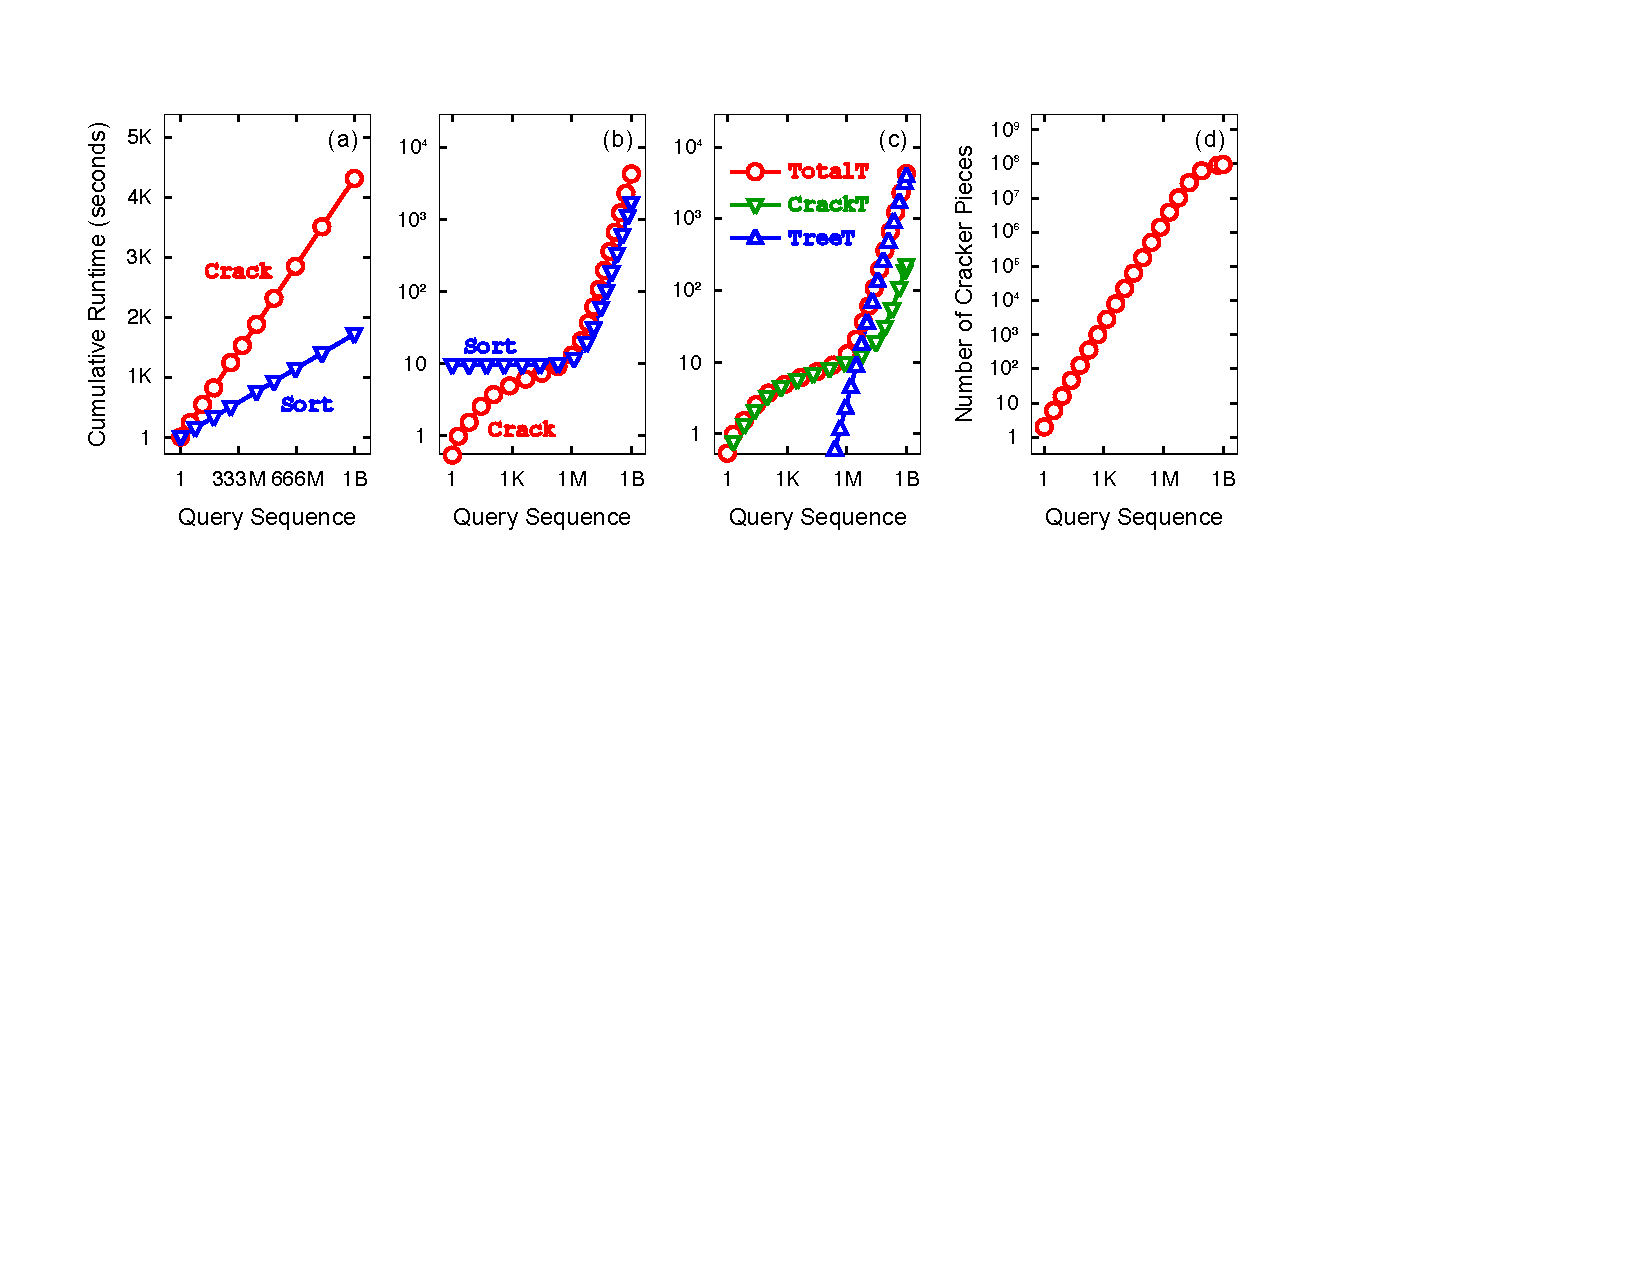
\includegraphics[width=1.5\columnwidth]{graphs/figure3.pdf}
\vspace{-2.5em}
\caption{Non-resilience during long query sequences.}
\vspace{-2em}
\label{F:LongSequenceProblem}
}
\hfill
\hspace{6.5em}%
\Fig[b]{.6\columnwidth}{%
\hspace{1.5em}%
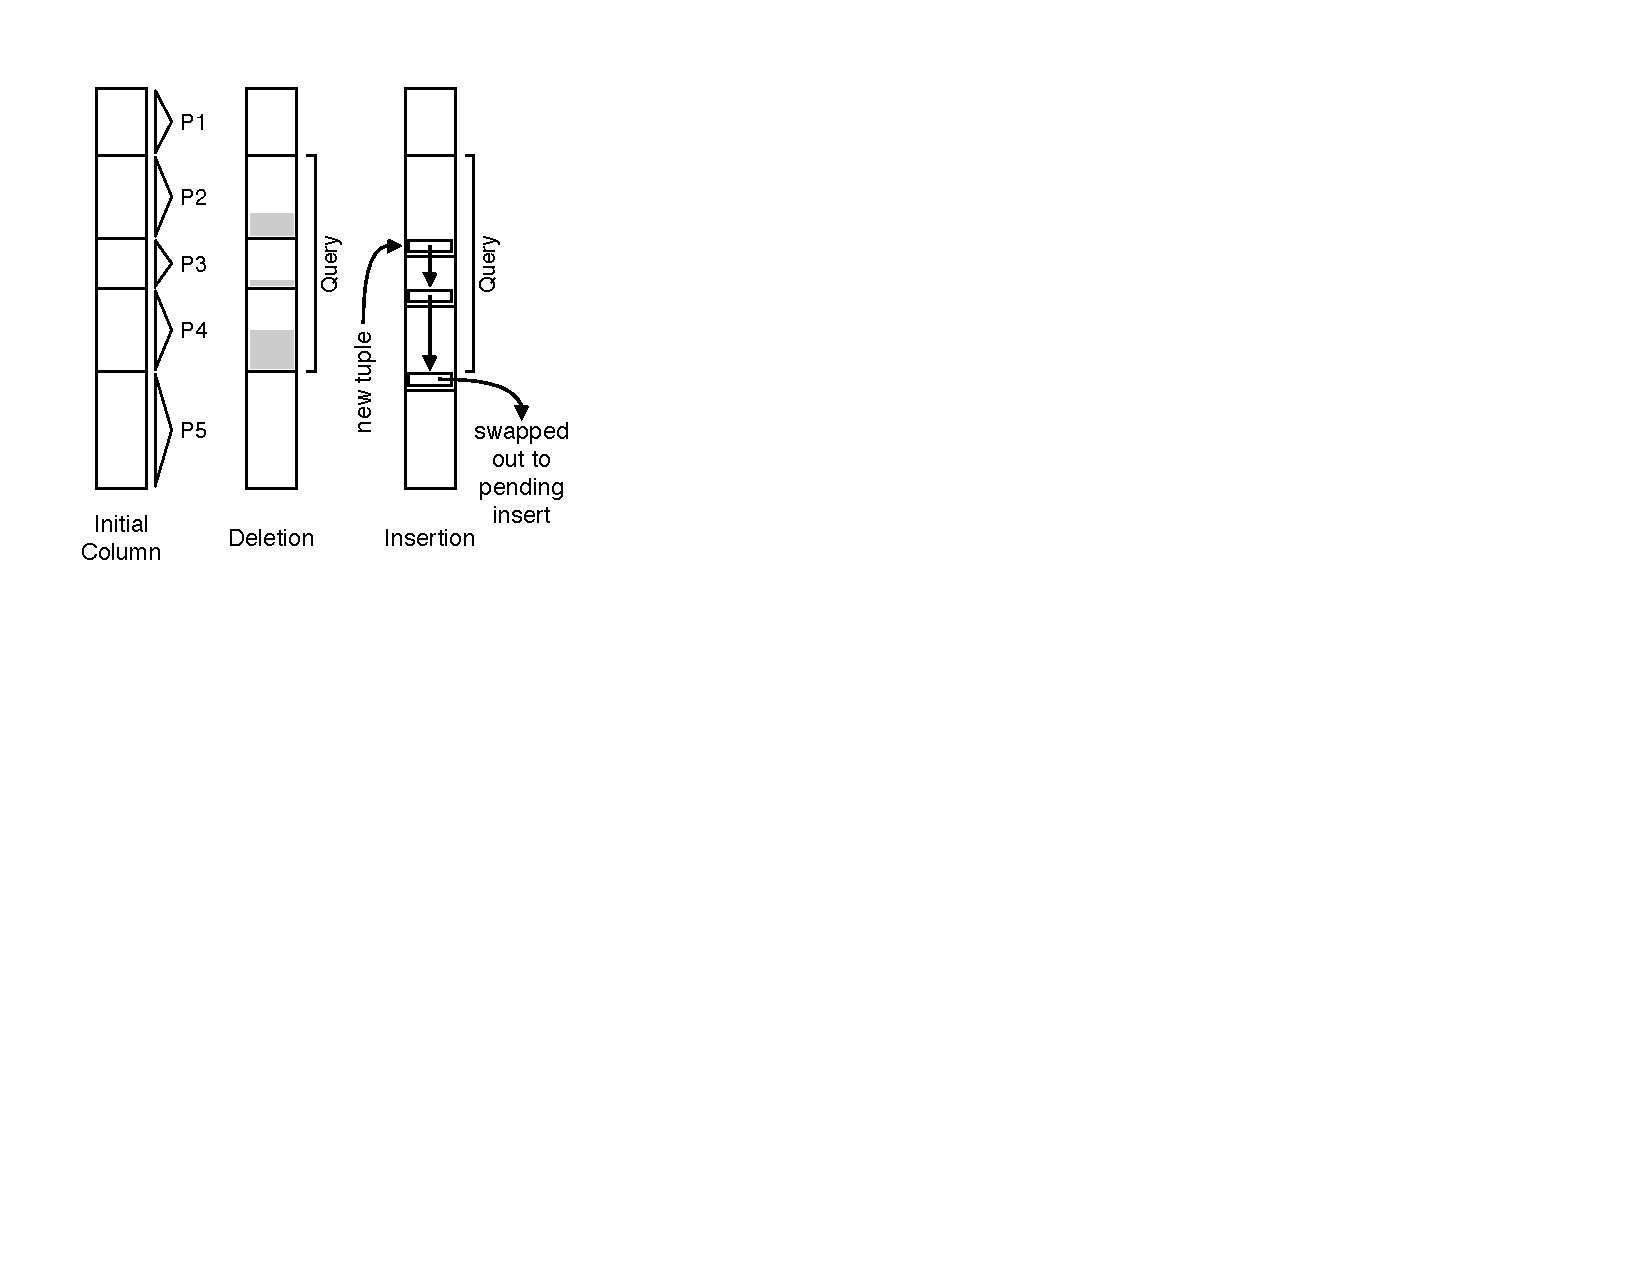
\includegraphics[width=.9\columnwidth]{graphs/fig_mrd_mri.pdf}%
\vspace{-1em}
\caption{Database cracking updates.}
\vspace{-2em}
\label{F:updates}
}
\end{figure*}


\textbf{Basic Cracking Performance.}
Figure \ref{F:BasicPerQuery}(a) shows a performance example where cracking is compared against
a full indexing approach ({\sf Sort}), in which we completely sort the column with the first query.
In an in-memory column-store, sorting a column creates the perfect index which allows for very fast
data access using binary search given that the underlying storage is 
fixed-width and dense arrays.
The data for this experiment consists of $10^8$ tuples of unique integers in $[0,2^{31})$.
The query workload is random -- the bounds are random while 
the ranges requested have a fixed selectivity of 1\% per query.
This scenario assumes a dynamic environment where there is no workload knowledge or idle time
in order to pre-sort the data, i.e., our very motivating example for adaptive indexing.


As Figure \ref{F:BasicPerQuery}(a) shows, once the data is sorted with the first query, from then on performance is
extremely fast as we only need to perform a binary search over the sorted column to satisfy each select operator request.
Nevertheless, the problem is that we overload the first query. On the other hand, database cracking
continuously improves performance without penalizing individual queries. Eventually, its performance reaches
the levels of {\sf Sort}.\
The benefit of cracking comes by continuously analyzing less and less data.
Figure \ref{F:BasicPerQuery}(b) shows the number of tuples each cracking query has to touch;
as we process more queries, more pieces are created by cracking the column and subsequent queries can 
reduce the amount of data touched by exploiting the more fine-grained index.

We also compare against a plain {\sf Scan} approach where data is always completely scanned. 
Naturally, as Figure \ref{F:BasicPerQuery}(a) shows, this has a stable behavior;
we observe that cracking does not significantly penalize any query more than the default {\sf Scan} approach.
Note, that while cracking and {\sf Sort} can simply return a view of the (contiguous)
qualifying tuples, {\sf Scan} has to materialize
a new array with the result. 

Figure \ref{F:BasicPerQuery}(c) shows the same results as in Figure \ref{F:BasicPerQuery}(a) but uses
a different metric; this time the graph plots the cumulative time as the query sequence evolves, i.e.,
every point $(x,y)$ depicts that it takes $y$ seconds in total to process the first $x$ queries.
Remarkably,  by the time cracking has already answered all $10^4$ queries
the full indexing approach still has not finished preparing the index. 
In dynamic environments with little idle time to invest in index preparation and with little knowledge
about which columns are actually interesting for the queries, adaptive indexing has a huge advantage.
Full offline indexing has no time to prepare and no intelligence  about which columns to index.
In the specific example in our experiment, if the workload changes sometime during those $10^4$ queries,
then full indexing is simply a waste of resources. 


\subsection{Problem 1: Long Query Sequences}
The previous discussion highlighted the main motivation and benefits of adaptive indexing.
Here, we expose the non-resilience problem when it comes to long exploratory query sequences.
We use a similar experiment as before with the same set-up;
the difference is that now we fire a significantly longer query sequence, i.e., up to 1 
billion queries as opposed to only $10^4$  queries we had before.

Figure \ref{F:LongSequenceProblem} shows the results, comparing cracking to full sorting.
Figure \ref{F:LongSequenceProblem}(a) depicts the cumulative response time.
It reveals that as the query sequence evolves, cracking loses its advantage over full sorting. 
The total cost for cracking at the end of the query sequence is more than 4000 seconds while 
full sorting needed less than half of that. The advantage of cracking early in the query sequence still remains. 
Figure \ref{F:LongSequenceProblem}(b) shows the same results with 
a log scale for both axes.
Up to roughly 1 million queries cracking enjoys a better performance. 
However, after this point, we reach a threshold where it would have been better to not use adaptive indexing
when considering the cumulative costs for the whole query sequence.

We analyze this behavior further by breaking down the cracking costs
in Figures \ref{F:LongSequenceProblem}(c) and (d). 
Figure \ref{F:LongSequenceProblem}(c) shows the total cracking costs (TotalT)
separated into the costs of searching the tree of the cracking index (TreeT) and to the cost of performing the actual cracking (CrackT),
i.e., the actual physical reorganization of the column. 
The cumulative time of these break-down metrics 
as the sequence evolves shows that
up to the threshold of 1 million queries the total query cost is dominated by the cracking costs of reorganizing the column.
However, after this point the cost is dominated by the cost of searching the tree.
Figure \ref{F:LongSequenceProblem}(d) verifies that searching the tree becomes the main bottleneck;
it plots the number of pieces in the cracking index. As we pose more queries, more pieces are created (at most 2 pieces per query)
and hence the tree grows and becomes more expensive to search due to random access.



\subsection{Problem 2: Continuous Data Updates}

Having seen the problem with long query sequences, we highlight 
an even more significant source of non-resilience
with existing adaptive indexing -- performance degradation in long sequences where 
updates interleave with queries.

\textbf{Cracking Updates.}
Let us first give a short description of how cracking performs updates as  proposed in \cite{IKM:SIGMOD07}.
To deal with updates, original cracking uses an adaptive approach. Updates (inserts or deletes)
are marked as pending updates upon arrival. For each column, there is a pending insertions and a pending deletions column.
Thus, update queries are  close to zero-cost queries as they do nothing more than appending the new updates at
the pending columns.
When read queries arrive, they on-the-fly merge any pending updates in the actual cracking columns.
They do so only for the updates that fall within the value range requested by the current query, enhancing the adaptive
behavior of cracking. If a range is never queried, then it is never updated.
The select operator is now responsible for both cracking and merging any qualifying updates at the proper cracking
pieces.
The merge actions do not destroy the cracker index, i.e., all the partitioning information is maintained.
Given that original cracking works on top of fixed-width and dense columns, it needs to ripple/shuffle values 
such that it can place new values in the proper pieces.
Figure \ref{F:updates} shows an example of how tuples need to be moved across pieces when inserting 
a new tuple or when removing an existing one.
Given that within each cracking piece values are not ordered, not all values within a piece need to be moved;
to move a full piece one position down, it is sufficient to move the first value of the piece to the end of this piece
and subsequently change the borders of the piece.
Deletes leave back holes, while a select operator makes sure that it ripples all holes at the borders of the piece
where they belong so that subsequent operators on this range can more easily go through the tuples of this piece. 
Holes are exploited to place new tuples in when possible.


\textbf{The Problem.}
To demonstrate the non-resilience problem in long sequences where
updates interleave with queries, 
we perform the same experiment as before; the difference now is that data is not static anymore.
Now data arrival events interleave with queries.
This scenario matches modern applications where data arrive periodically  but quite often, i.e., 
every few hours or minutes, while we still want to explore the data for interesting patterns in online manner.
The set-up is the same as in the previous experiment;
the difference here is that every  10 read queries, 10 random insert queries and 10 random delete queries arrive.

Figure \ref{F:UpdatesProblem} shows the results for cracking as the query sequence evolves.
Figure \ref{F:UpdatesProblem}(a) shows that after about $10^4$ queries the 
cumulative total cost (TotalT) grows significantly. 
Figure \ref{F:UpdatesProblem}(a) also breaks this cost down to the cost that each query spends
to merge any updates (InsertT), to merge any deletes (DeleteT) and to the actual cracking cost to reorganize the 
column (CrackT). After $10^4$ queries the cost to merge the insertions becomes the dominant component and overshadows
the cracking costs by two orders of magnitude.
Figure \ref{F:UpdatesProblem}(b) depicts the amount of tuples examined as the query sequence evolves 
and the kind of actions performed. 
It shows that as we process more queries, significantly more tuples need to be touched.
In particular, significantly more tuples need to be rippled, i.e., they need to be moved into a new position
in the column. After $10^4$ queries, it is this action that dominates the actions performed and thus the total cost.
As more pieces are created, more data movement is needed in order to maintain
the partitioning information in the index. In this way, as the sequence evolves, performance degrades
due to the excessive update and administration costs.

Comparing Figure \ref{F:UpdatesProblem}(a) to 
Figure \ref{F:LongSequenceProblem}(b) (where we had no updates), we see that the performance
degradation occurs much earlier when updates interleave with queries, 
i.e., after only $10^4$ queries versus after $10^6$ queries in the read only scenario. 






